\chapter{Experiment 1}
Bei der ersten Forschungsfrage soll überprüft werden, wie sich eine durch Reinforcement Learning erlernte Policy mit der Policy der Heuristik vergleicht, welche in \autoref{sec:ff} beschrieben wurde.
\section{Beschreibung}
\label{sec:exp1-desc}
Um die erste Forschungsfrage empirisch zu beantworten, bedarf es eines geregelten Vorgehens. Es werden zwei durch unterschiedliche Reinforcement Learning-Algorithmen optimierte Policies mit der Policy der Heuristik verglichen. Diese werden einmal durch Sarsa und einmal durch Q-Learning gelernt. Um zwei optimierte Policies zu erlernen, müssen die Parameter gewählt werden, welche den Reward einer Policy maximieren. Dazu werden verschiedene Durchgänge ausgeführt, bei denen jeweils nur ein Parameter angepasst wurde.
 \begin{figure}[H]
 \centering
  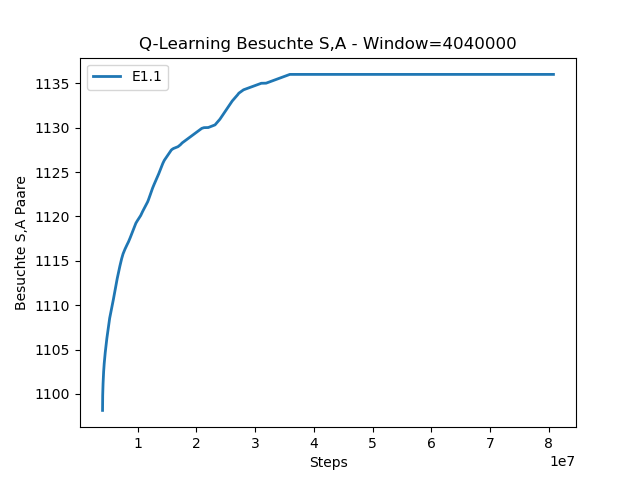
\includegraphics[height=5.5cm]{img/plots/exp-1/visited_800k.png}
  \caption{SA-Paare – Zufällige Actions 800'000 Episoden}
      \label{fig:visited_800k}
\end{figure}
Um sicherzustellen, dass sämtliche möglichen State-Action-Paare besucht werden, wurde ein rein explorativer Agent für 800'000 Episoden aufgeführt. In Abbildung \ref{fig:visited_800k} ist ersichtlich, wie nach ungefähr 400'000 Episoden 1136 State-Action-Paare besucht wurden. In der zweiten Hälfte wurden dabei keine weiteren States gefunden, woraus sich schliessen lässt, dass keine weiteren State-Action-Paare erreichbar sind. Um die Parameter zu prüfen, werden jeweils 50'000 Episoden durchgeführt. Diese garantieren nicht, dass jedes State-Action-Paar besucht wurde, da dies bei einem Agent, der zufällige Actions wählt, erst nach ungefähr 400'000 Episoden der Fall ist. Sie geben aber bereits einen hilfreichen Eindruck, welche Parameter besser geeignet sind. Die Policies mit den richtigen Parametern werden aber anschliessend mit 800'000 Episoden erlernt. Ausserdem wird überprüft, ob die 1136 State-Action-Paare erreicht wurden. 
\subsection{Exploration}
Als Erstes wird die Exploration untersucht. Der Explorationswert $\epsilon$ wird zu Beginn bei 1 festgelegt und über die Zeit mit einem Faktor, dem Epsilon-Verfall, verringert, bis ein Minimum von 0.05 erreicht wird. Dadurch soll sichergestellt werden, dass am Ende immer noch eine 5-prozentige Chance besteht, dass eine zufällige Action gewählt wird. Es werden unterschiedliche Werte für den Epsilon-Verfall gewählt und untersucht. Hierbei wird versucht, möglichst kurz zu explorieren, aber sicherzustellen, dass eine optimale Policy gefunden wird und der Agent nicht bei einem lokalen Optimum verbleibt. Dazu wird verglichen, nach wie vielen Steps wie viele States besucht wurden. Dabei wird im Durchgang 1.5 ein Verfall von 1 gewählt, um so ein rein exploratives Vorgehen zu erzwingen. Ein Parameter möglichst nah an 1, welcher noch genügend Episoden zum Optimieren übriglässt, wäre ideal. Folgende Parameter werden geprüft:
\begin{table}[H]%
\begin{tabularx}{\textwidth} { 
  | >{\raggedright\arraybackslash}X 
  | >{\raggedright\arraybackslash}X 
  | >{\raggedright\arraybackslash}X
  | >{\raggedright\arraybackslash}X|}
 \hline
  Durchgang &Discount-Factor $\gamma$ &Lernrate $\alpha$ &$\epsilon$-Verfall\\
\hline
 E1.1&	0.9	&0.5	&\textbf{0.9985}\\
 \hline
  E1.2&	0.9	&0.5	&\textbf{0.9990}\\
 \hline
  E1.3&	0.9	&0.5	&\textbf{0.9995}\\
 \hline
  E1.4&	0.9	&0.5	&\textbf{0.9999}\\
 \hline
  E1.5&	0.9	&0.5	&\textbf{1}\\
 \hline
\end{tabularx}
\caption{Experiment 1 – Epsilon-Verfall}
\end{table}%
\newpage
\subsection{Discount-Factor}
Der Discount-Factor $\gamma$ definiert, wie stark zukünftige Rewards gewertet werden. Ein \\ Discount-Factor von 0 bedeutet, dass der Agent ausschliesslich auf den aktuellen Reward achtet. Im Gegensatz dazu sagt ein Wert 1 aus, dass sämtliche zukünftigen Rewards berücksichtigt werden. Folgende Parameter werden geprüft:
\begin{table}[H]%
\begin{tabularx}{\textwidth} { 
  | >{\raggedright\arraybackslash}X 
  | >{\raggedright\arraybackslash}X 
  | >{\raggedright\arraybackslash}X
  | >{\raggedright\arraybackslash}X|}
 \hline
  Durchgang &Discount-Factor $\gamma$ &Lernrate $\alpha$ &$\epsilon$-Verfall\\
\hline
 G1.1&	\textbf{0.9}	&0.5	&0.999\\
 \hline
  G1.2&	\textbf{0.8}	&0.5	&0.999\\
 \hline
  G1.3&	\textbf{0.7}	&0.5	&0.999\\
 \hline
  G1.4&	\textbf{0.6}	&0.5	&0.999\\
 \hline
  G1.5&	\textbf{0.5}	&0.5	&0.999\\
 \hline
\end{tabularx}
\caption{Experiment 1 – Discount-Factor}
\end{table}%

\subsection{Lernrate}
Die Lernrate $\alpha$ definiert, wie schnell die Q-Values auf neue Erkenntnisse angepasst werden. Ein Wert von 0 bedeutet, es wird nichts dazugelernt, und der Wert 1 heisst, dass der komplette TD-Error ausgeglichen wird. Folgende Lernraten werden überprüft:
\begin{table}[H]%
\begin{tabularx}{\textwidth} { 
  | >{\raggedright\arraybackslash}X 
  | >{\raggedright\arraybackslash}X 
  | >{\raggedright\arraybackslash}X
  | >{\raggedright\arraybackslash}X|}
 \hline
  Durchgang &Discount-Factor $\gamma$ &Lernrate $\alpha$ &$\epsilon$-Verfall\\
\hline
 A1.1&	0.9	&\textbf{0.5}	&0.999\\
 \hline
  A1.2&	0.9	&\textbf{0.6}	&0.999\\
 \hline
  A1.3&	0.9	&\textbf{0.7}	&0.999\\
 \hline
  A1.4&	0.9	&\textbf{0.8}	&0.999\\
 \hline
  A1.5&	0.9	&\textbf{0.9}	&0.999\\
 \hline
\end{tabularx}
\caption{Experiment 1 – Lernrate}
\end{table}%

\newpage
\subsection{Messwerte}
Der Messwert, mit welchem die Policies verglichen werden, ist der Reward. Dazu wird der mittlere Reward der letzten 50 Episoden verwendet; ausserdem wird dieser Wert noch durch 100 dividiert, um somit den mittleren Step-Reward pro Episode zu erhalten. Der mittlere Step-Reward ist deshalb interessant, da man diesen mit einem optimalen Wert vergleichen kann. Es werden alle 4 Steps Aufträge generiert, und somit wäre ohne Lagerkosten pro Step ein Reward von 25 das Maximum.
Zuerst werden in einem direkten Vergleich die beiden Algorithmen gegenübergestellt. Dadurch soll ersichtlich sein, welcher Algorithmus einen höheren Reward erreicht und überprüft werden, ob sämtliche State-Action-Paare besucht wurden.
In einem zweiten Schritt wird nun noch die erlernte Policy der Algorithmen direkt auf einen Agent übertragen, welcher jeweils ohne Exploration die beste Action auswählt. Somit kann ein fairer Vergleich mit denselben Bestellungen angestellt werden. Dabei ist zu erwarten, dass die Policies ein konstantes Ergebnis über die Episoden erreichen, da mit nur einem Artikel kein Zufall im Environment vorhanden ist.
Die Werte in den Diagrammen werden, um die Übersichtlichkeit zu erhöhen, über eine bestimmte Anzahl an Werten, das sogenannte Window, gemittelt.
\smallskip\\
\begin{figure}[hb]
  \centering
  \href{https://github.com/benji24290/rl-warehouse/tree/experiment_1}{
\includegraphics[height=1.9cm]{img/qr/qrcode_exp1.jpeg}}
  \caption{Experiment 1 – Link}
\end{figure}
\newpage
\section{Resultate}
Im ersten Experiment, welches in \ref{sec:exp1-desc} definiert ist, wurde als Erstes die Exploration untersucht. Dabei konnte geprüft werden, welcher Epsilon-Verfall am besten geeignet ist. Der Wert 0.9999 aus Durchgang E1.4 erweist sich bei beiden Algorithmen als gut geeignet, da die State-Action-Paare am schnellsten erreicht werden und bereits ab 30'000 Episoden nur noch mit dem Minimum exploriert wird. Dadurch hat der Agent noch die restlichen Episoden Zeit, die Q-Values der State-Action-Paare zu optimieren. Bei 800'000 Episoden muss das entsprechende Epsilon angepasst werden, was gerundet ungefähr einem Epsilon-Verfall von 0.9999938 entspricht.
\begin{figure}[H]
\centering
  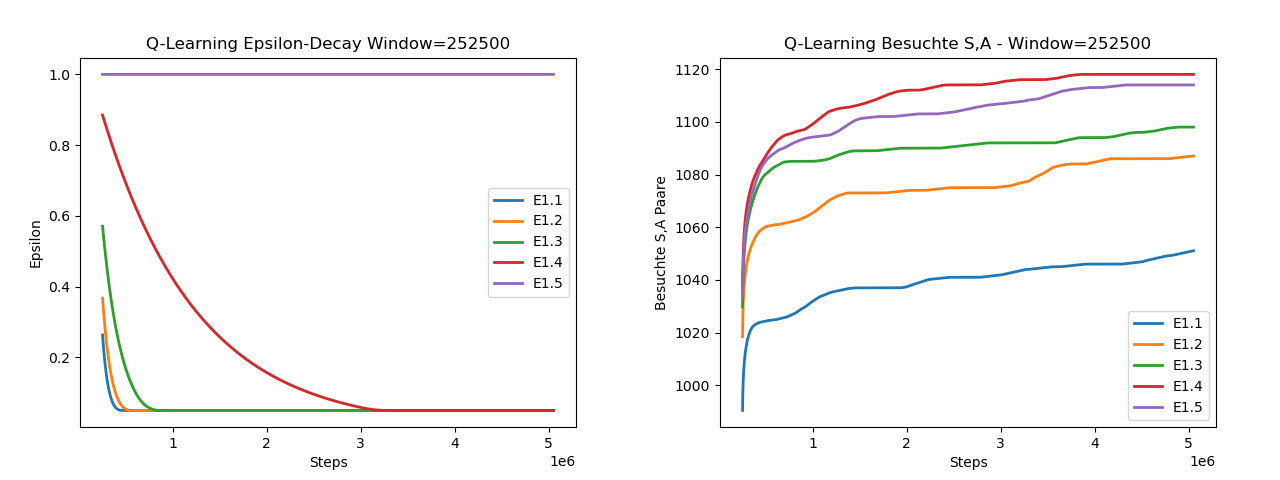
\includegraphics[height=5.5cm]{img/plots/exp-1/Exploration_Q.png}
  \caption{Experiment 1 – Exploration Q-Learning}
    \label{fig:e1-expl-q}
\end{figure} 
\begin{figure}[H]
\centering
  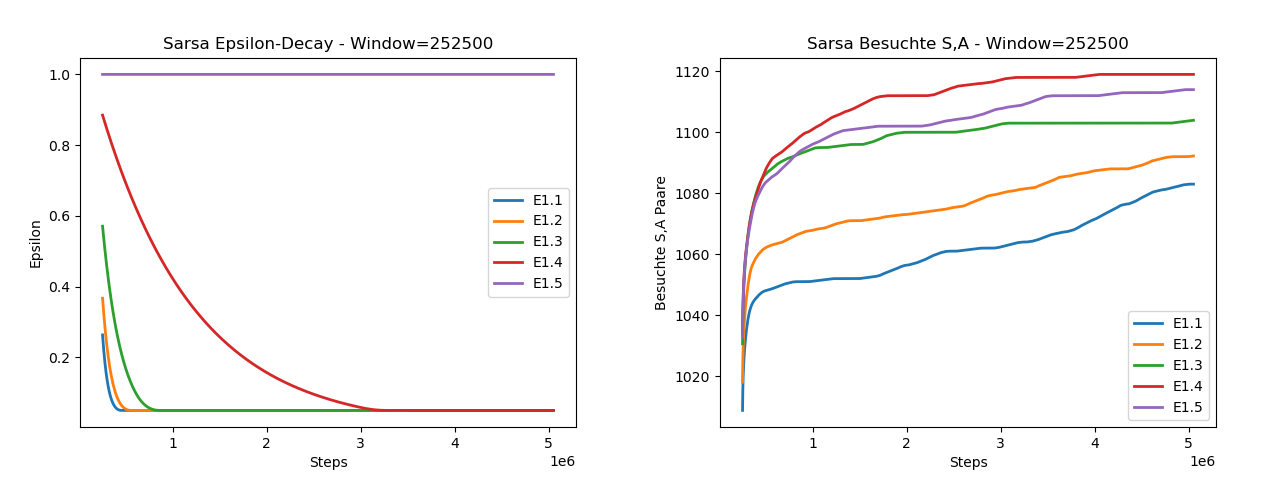
\includegraphics[height=5.5cm]{img/plots/exp-1/Exploration_Sarsa.png}
  \caption{Experiment 1 – Exploration Sarsa}
    \label{fig:e1-expl-q}
\end{figure} 

In Tabelle \ref{tab:e1-res-alpha} sind die Ergebnisse aus dem Parametervergleich für die Lernrate ersichtlich. Hierbei wurde jeweils der durchschnittliche Step-Reward der letzten 50 Episoden berechnet. Dabei ist erkennbar, dass die beiden Algorithmen jeweils mit unterschiedlichen Lernraten am besten performen. Für Q-Learning wird beim finalen Trainieren eine Lernrate von 0.9 und bei Sarsa 0.6 verwendet; diese haben in Tabelle \ref{tab:e1-res-alpha} jeweils den höchsten Step-Reward erzielt.
\begin{table}[H]%
\begin{tabularx}{\textwidth} { 
  | >{\raggedright\arraybackslash}X 
  | >{\raggedright\arraybackslash}X 
  | >{\raggedright\arraybackslash}X
  | >{\raggedright\arraybackslash}X|}
 \hline
  Durchgang &Lernrate &Q-Learning &Sarsa\\
\hline
 A1.1&0.5	&16.18 &14.71\\
 \hline
  A1.2&0.6	&18.26 &\textbf{17.22}\\
 \hline
  A1.3&0.7	&18.14 &15.16\\
 \hline
  A1.4&0.8	&18.02 &13.14\\
 \hline
  A1.5&0.9 &\textbf{19.42} &10.84\\
 \hline
\end{tabularx}
\caption{Experiment 1 – Resultate Lernrate}
\label{tab:e1-res-alpha}
\end{table}%

Zuletzt wurde der Discount-Factor überprüft. Dabei wurde auch der durchschnittliche Step-Reward aus den letzten 50 Episoden errechnet. Aus Tabelle \ref{tab:e1-res-gamma} wird ersichtlich, dass Q-Learning mit einem Gamma von 0.8 und Sarsa mit einem Gamma von 0.6 am besten performen.

\begin{table}[H]%
\begin{tabularx}{\textwidth} { 
  | >{\raggedright\arraybackslash}X 
  | >{\raggedright\arraybackslash}X 
  | >{\raggedright\arraybackslash}X
  | >{\raggedright\arraybackslash}X|}
 \hline
  Durchgang &Discount-Factor &Q-Learning &Sarsa\\
\hline
 G1.1&0.9	&16.18 &14.71\\
 \hline
  G1.2&0.8	&\textbf{17.45} &17.26\\
 \hline
  G1.3&0.7	&16.47 &16.01\\
 \hline
  G1.4&0.6	&18.02 &\textbf{18.43}\\
 \hline
  G1.5&0.5 &15.55 &17.93\\
 \hline
\end{tabularx}
\caption{Experiment 1 – Resultate Discount-Factor}
\label{tab:e1-res-gamma}
\end{table}%
\newpage
Nach den drei Durchgängen, in denen jeweils die besten Parameter für die beiden Algorithmen gewählt wurden, wird nun während 800'000 Episoden versucht, eine optimale Policy zu erlernen. Dabei ist in Abbildung \ref{fig:e1-train} zu sehen, dass Q-Learning einen höheren durchschnittlichen Reward erreicht als Sarsa. Der transparente Bereich zeigt die Varianz des Rewards. Der $TDError^2$, welcher aus Abbildung \ref{fig:e1-train} hervorgeht, hat bei beiden Algorithmen nach etwa 500'000 Episoden konvergiert. Der Grund dafür ist das Epsilon, welches – wie Abbildung \ref{fig:e1-expl-both} zeigt – nach dieser Anzahl an Episoden auf dem Minimum von 0.05 angekommen ist. Ausserdem erkennt man, wie Q-Learning, im Gegensatz zu Sarsa, die Anzahl der erreichbaren State-Action-Kombinationen bereits kurz vor 600'000 Episoden (Abbildung \ref{fig:e1-expl-both}) erreicht hat.
\begin{figure}[H]
  \centering
  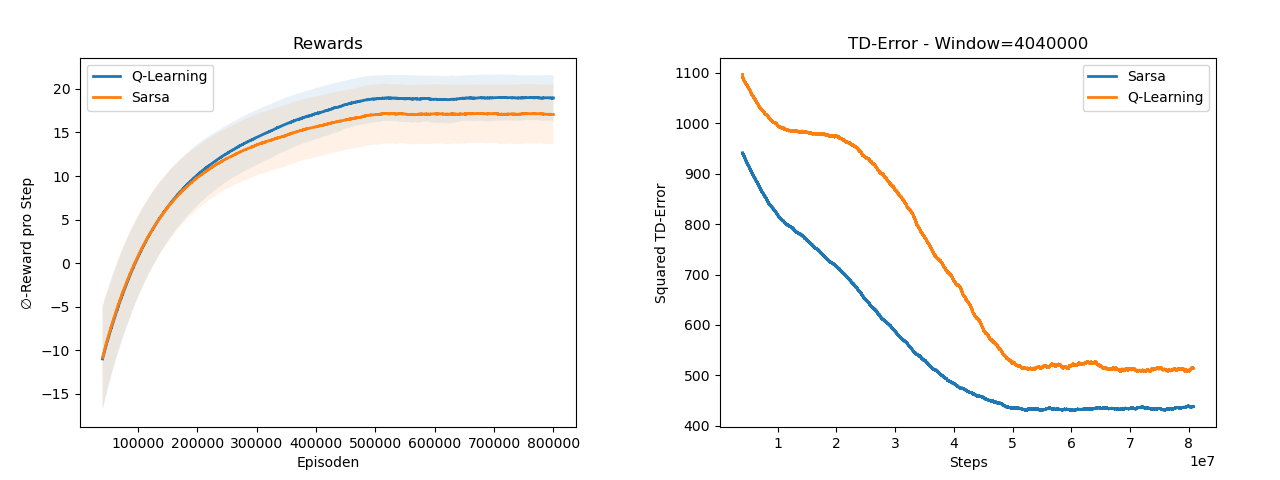
\includegraphics[height=5.5cm]{img/plots/exp-1/train.png}
  \caption{Experiment 1 – Reward und TD-Error}
    \label{fig:e1-train}
\end{figure} 
\begin{figure}[H]
  \centering
  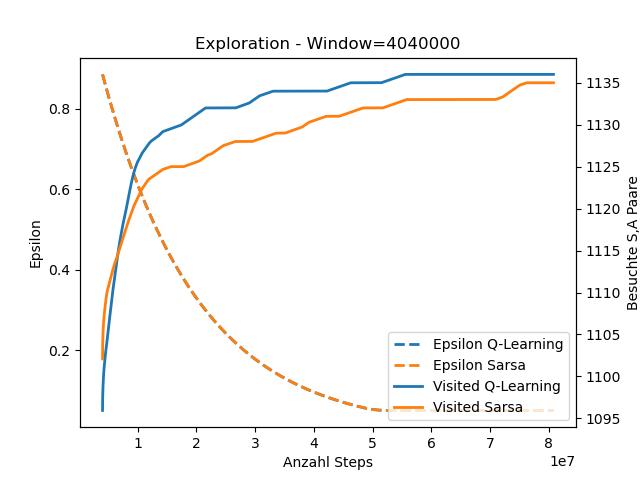
\includegraphics[height=5.5cm]{img/plots/exp-1/both_exploration.png}
  \caption{Experiment 1 – Exploration}
    \label{fig:e1-expl-both}
\end{figure}
In der folgenden Abbildung \ref{fig:e1-reward-freq} ist ersichtlich, wie oft ein gewisser Reward in der jeweiligen Episode verteilt wurde. Für negative Rewards wurde die Anzahl invertiert. Dabei ist zu erkennen, wie die Algorithmen die negativen Rewards, wie die für das Stornieren, für eine volle Ankunft oder eine falsche Auslieferung minimieren. Auch die Lagerkosten werden versucht auf das Nötigste zu minimieren. Nur die gelungenen Auslieferungen pro Episode haben mit steigender Anzahl an Episoden zugenommen.
\begin{figure}[H]
  \centering
  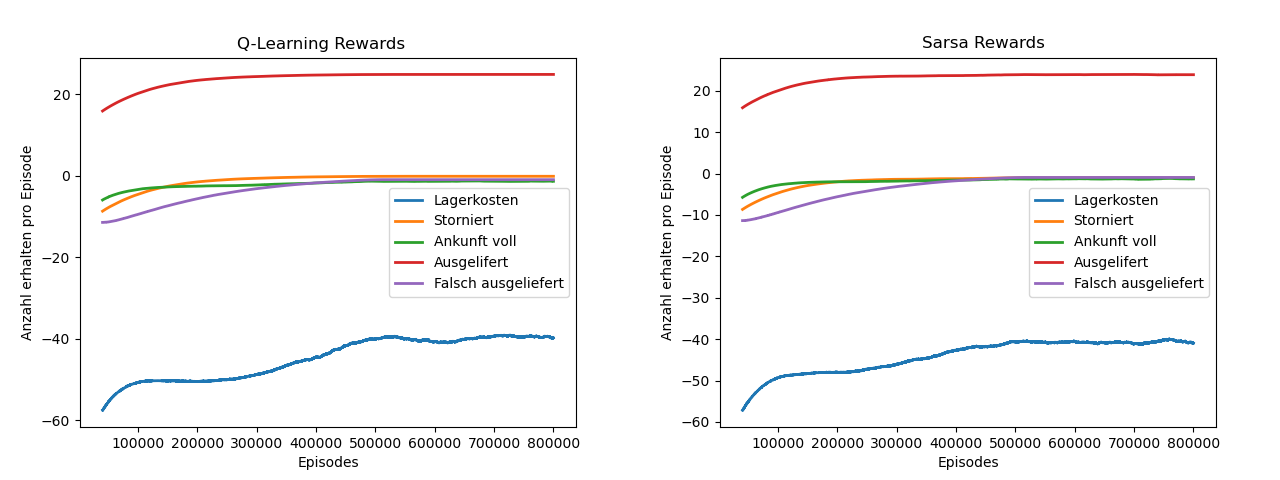
\includegraphics[height=5.3cm]{img/plots/exp-1/reward_frequency.png}
  \caption{Experiment 1 – Vorkommen der Rewards pro Step (Window = 40'400)}
    \label{fig:e1-reward-freq}
\end{figure}
Mit dem erfolgreichen Trainieren der Policies steht nun eine Q-Matrix zur Verfügung, die an einen Greedy-Agent übergeben wird. Dieser Agent wählt ausschliesslich die Action, welche den höchsten Q-Value für einen gegebenen State aufweist. Wie erwartet, ist in Abbildung \ref{fig:e1-comp-policies} zu erkennen, dass die Policies über die 1000 Episoden jeweils denselben Reward erzielen. Das ist korrekt, da in Experiment 1 nur ein Artikel und somit in jeder Episode dasselbe Sample an Aufträgen entsteht.
\begin{figure}[H]
  \centering
  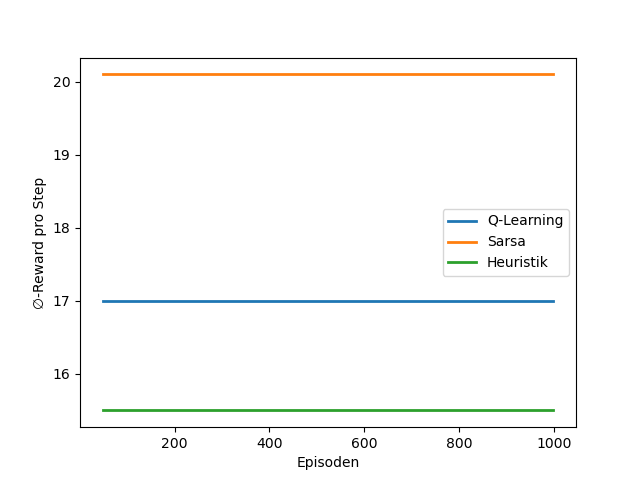
\includegraphics[height=5.2cm]{img/plots/exp-1/Compare.png}
  \caption{Experiment 1 – Vergleich der Policies}
    \label{fig:e1-comp-policies}
\end{figure}

In diesem Experiment hat Sarsa den mittleren Step-Reward der heuristischen Policy um 30 Prozent übertroffen (Tabelle \ref{tab:e1-res-poli}).
\begin{table}[H]%
\begin{tabularx}{\textwidth} { 
  | >{\raggedright\arraybackslash}l 
  | >{\raggedright\arraybackslash}X 
  | >{\raggedright\arraybackslash}X
  | >{\raggedright\arraybackslash}X|}
 \hline
  Policy &Q-Learning &Sarsa &Heuristik\\
\hline
 Ø-Step-Reward&17.0	&20.1 &15.5\\
 \hline
  Vergleich zur Heuristik&+9.7\%	&+29.7\% &+0\%\\
 \hline
\end{tabularx}
\caption{Experiment 1 – Resultate Policies}
\label{tab:e1-res-poli}
\end{table}%

In den folgenden Abbildungen \ref{fig:e1-pol-heu}, \ref{fig:e1-pol-q} und \ref{fig:e1-pol-sarsa} wurde für jeden Agent dieselbe Episode ausgewählt und die erreichten Rewards sowie der State dieser Episode wurden dargestellt. Diese Darstellungen ermöglichen es, die Unterschiede der Agents besser aufzuzeigen.
Abbildung \ref{fig:e1-pol-heu} zeigt die Rewards der Heuristik für eine Episode. Wie man erkennen kann, verpasst diese Policy jede 5. Bestellung. Dieses Resultat ist nachvollziehbar, denn die definierte Heuristik hält nur ein Exemplar pro Artikel auf Lager und das Bestellen bis zum Ausliefern dauert 5 Steps. Es werden jedoch alle 4 Steps Aufträge generiert.

\begin{figure}[H]
  \centering
  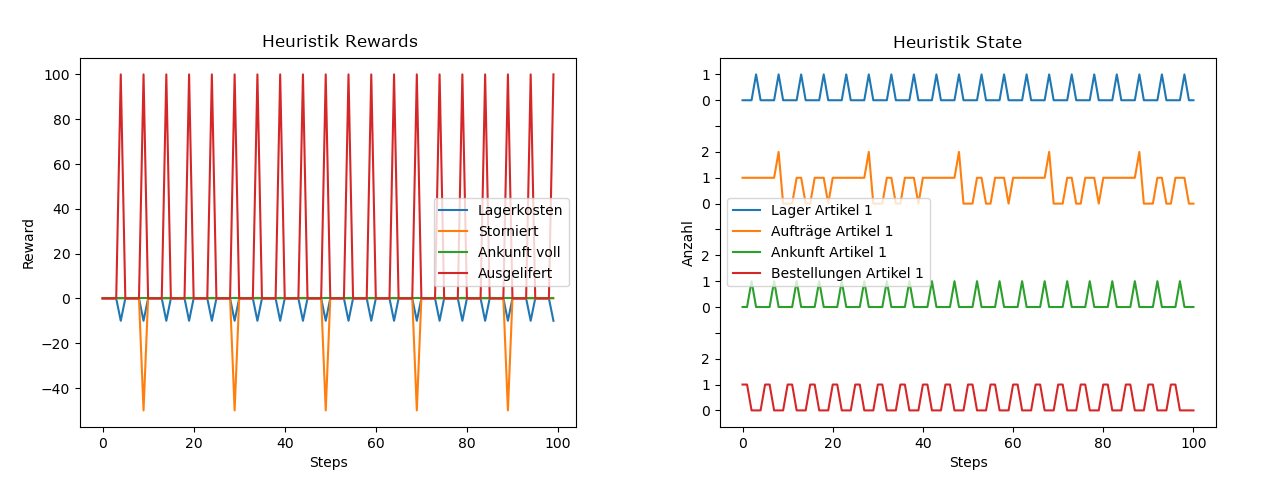
\includegraphics[height=5.5cm]{img/plots/exp-1/heu-rew-state.png}
  \caption{Experiment 1 – Rewards und States aus einer Episode Heuristik}
    \label{fig:e1-pol-heu}
\end{figure}

\newpage
Wie in Abbildung \ref{fig:e1-pol-q} erkennbar, hat die Q-Learning-Policy versucht, die Lagerplätze durch den Wareneingang zu ersetzen, da dieser im Environment keine Kosten generiert. Da aber zu viele Artikel im Eingang sind, wird trotzdem ein negativer Reward verteilt. 

\begin{figure}[H]
  \centering
  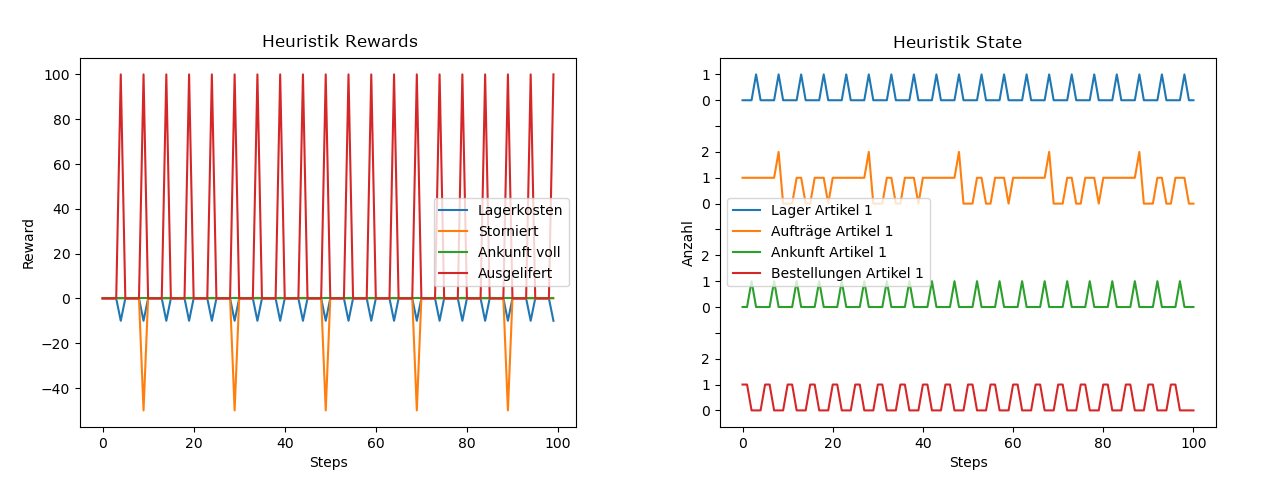
\includegraphics[height=5.5cm]{img/plots/exp-1/heu-rew-state.png}
  \caption{Experiment 1 – Rewards und States aus einer Episode Q-Learning}
    \label{fig:e1-pol-q}
\end{figure}
Sarsa hingegen hat gelernt, dass nur zu Beginn zwei Bestellungen nacheinander vorkommen und bestellt diese demensprechend (Abbildung \ref{fig:e1-pol-sarsa}). Dieses Vorgehen entspricht einem Overfitting, was in diesem Fall das Auswendiglernen einer bestimmten Sequenz bedeutet. Da das Environment aber immer gleich bleibt und keine zufälligen Abläufe stattfinden, ist das in diesem Fall die beste Policy.
\begin{figure}[H]
  \centering
  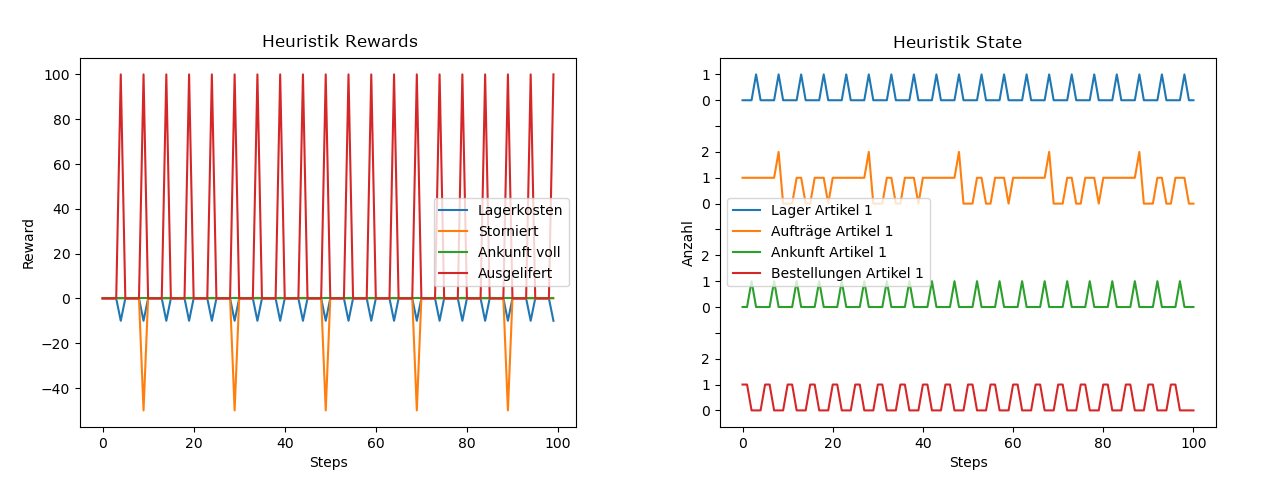
\includegraphics[height=5.5cm]{img/plots/exp-1/heu-rew-state.png}
  \caption{Experiment 1 – Rewards und States aus einer Episode Sarsa}
    \label{fig:e1-pol-sarsa}
\end{figure}